\documentclass{beamer}

\title{Consumers as Tax Auditors}
\author{Joana Naritomi}
\date{\today}

\begin{document}

\frame{\titlepage}

\begin{frame}
\frametitle{Introduction}
\begin{itemize}
\item We discussed in an earlier class that tax enforcement is crucial. You just not only need to detect but also recover evasion. 
\item However, changes in tax enforcement effectively increase effective tax rates as reporting increases. Therefore, there can be a trade off between tax enforcement vs tax rates.
\item If you need to raise R new dollars, either increase enforcement or increase tax rates
\item In Jensen paper we discussed that imperfect enforcement through informality can be redistributive, therefore it might be sometimes better to increase taxes rather than enforcement.
\end{itemize}
\end{frame}

\begin{frame}
\frametitle{This paper}
\begin{itemize}
    \item How tax enforcement and tax rates jointly effect fiscal capacity in low income countries? 
    \item Randomly assign 38,028 property owners to the status quo tax rate or to a rate reduction.
    \item Changes in reported tax liabilities indicate that current rate was above revenue maximizing threshold. 
    \item Then, through randomized enforcement
letters and random assignment of tax collectors shows that the RMTR increases with enforcement. 
\item Tax rates and enforcement are thus complementary levers. 
  
\end{itemize}
\end{frame}

\begin{frame}{Empirical Approach}
\begin{itemize}
    \item Compare retail firms vs wholesalers. 
    \item Reported revenue by retail firms increased by 21\% within 4 years of reform. This is likely a lower bound.
    \item Study mechanisms through winners of lottery and volume of firm sales or mass of consumers of a firm. 
\end{itemize}
\end{frame}

\begin{frame}{First Stage}
\begin{figure}
    \centering
    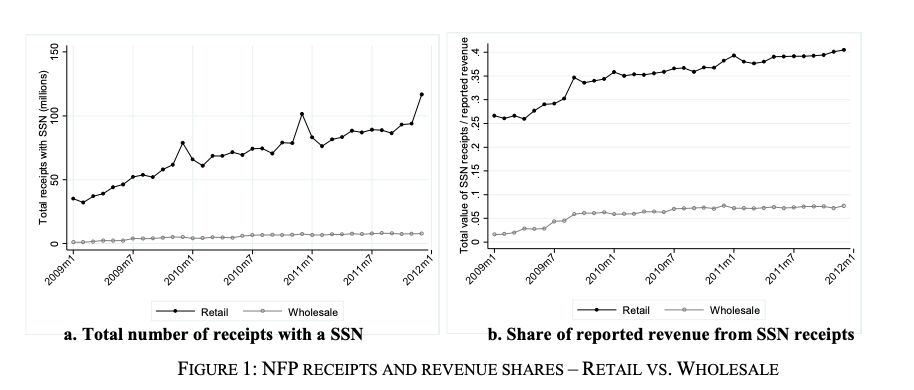
\includegraphics[width=\textwidth]{Paper Presentations/Consumers as Tax Auditors/F1.png}
    \label{fig:enter-label}
\end{figure}
\end{frame}

\begin{frame}{Effect of Reform}
\begin{figure}
    \centering
    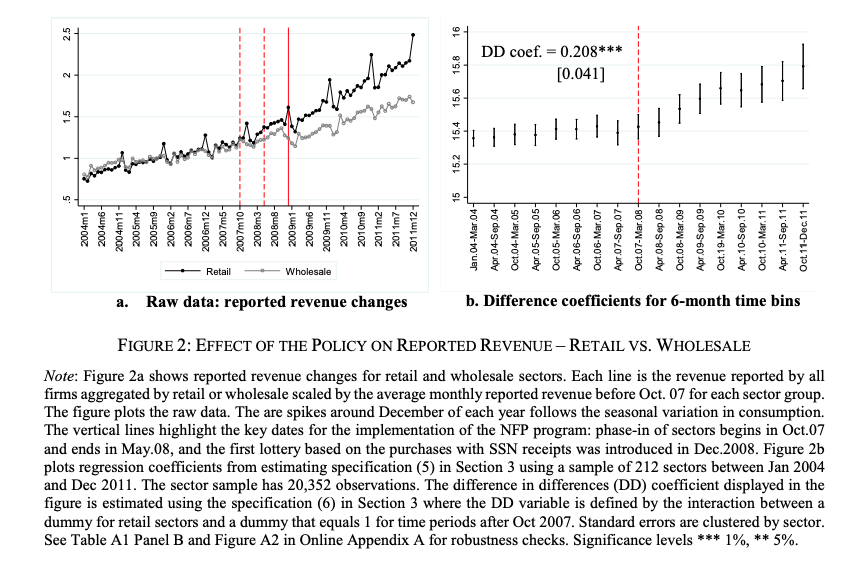
\includegraphics[width=\textwidth]{Paper Presentations/Consumers as Tax Auditors/Impact.png}
    \label{fig:enter-label}
\end{figure}
\end{frame}

\begin{frame}{Who responds to the reform?}
\begin{figure}
    \centering
    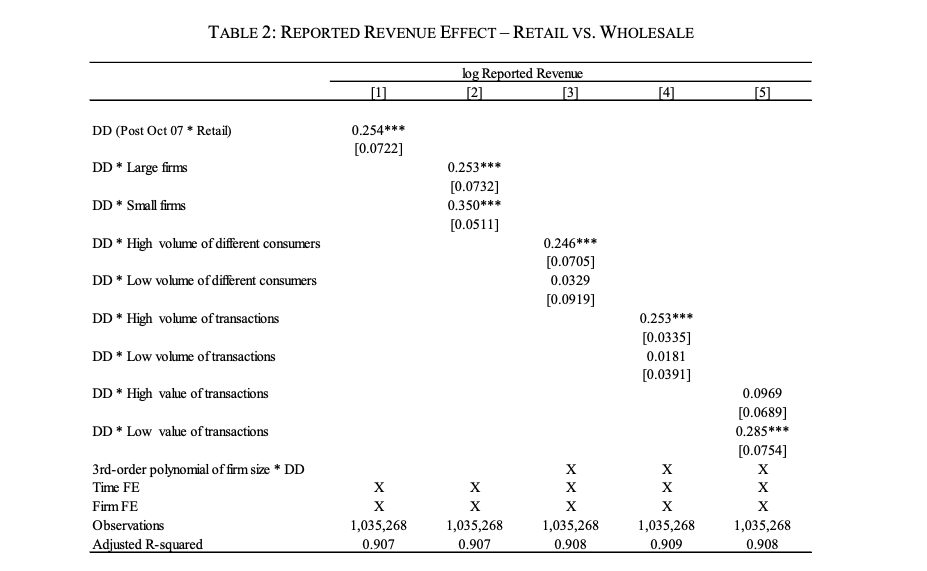
\includegraphics[width=\textwidth]{Paper Presentations/Consumers as Tax Auditors/T1.png}
    \label{fig:enter-label}
\end{figure}
\end{frame}

\begin{frame}{Do they deduct more?}
\begin{figure}
    \centering
    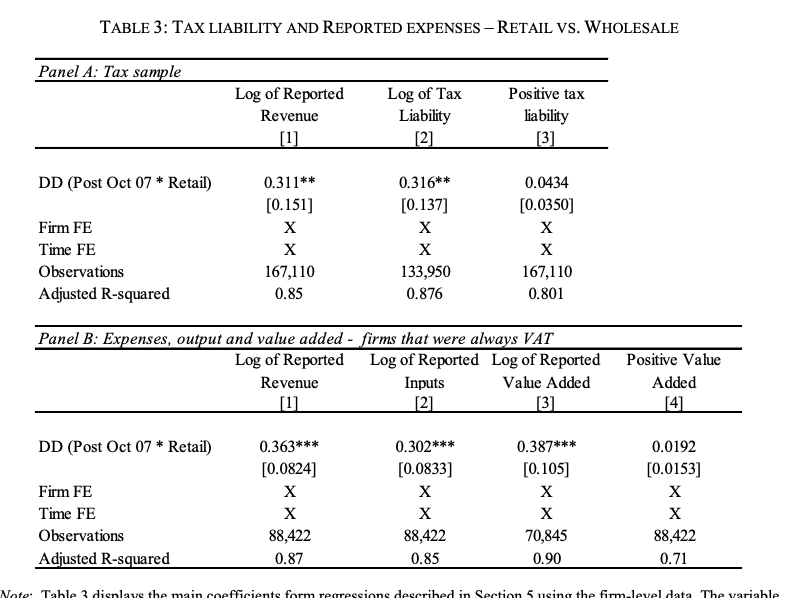
\includegraphics[width=\textwidth]{Paper Presentations/Consumers as Tax Auditors/T2.png}
    \label{fig:enter-label}
\end{figure}
\end{frame}



\begin{frame}
\frametitle{Taxes go up}
\begin{figure}
    \centering
    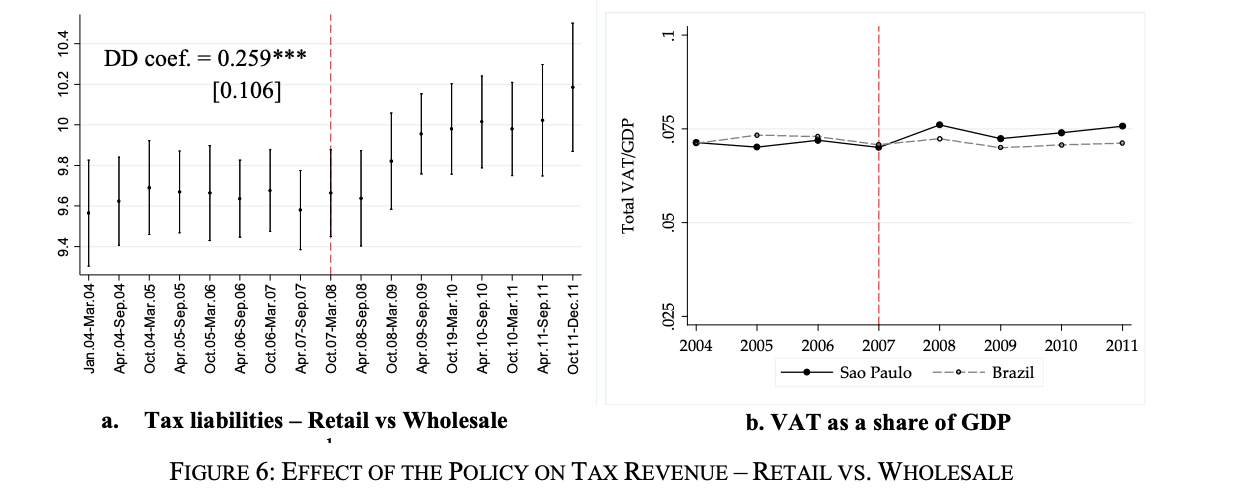
\includegraphics[width=\textwidth]{Paper Presentations/Consumers as Tax Auditors/TEPOLICY.png}
\end{figure}
\end{frame}

\begin{frame}{Effect of Whistle Blowers}
\begin{figure}
    \centering
    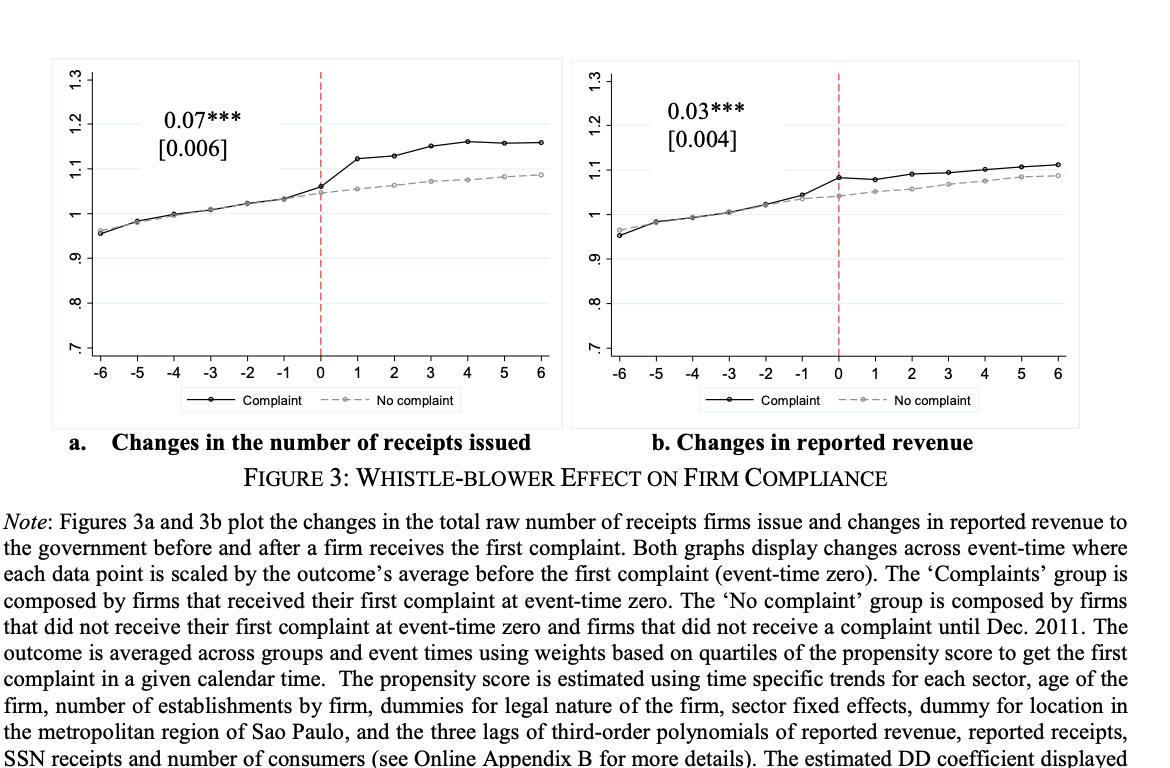
\includegraphics[width=\textwidth]{Paper Presentations/Consumers as Tax Auditors/Whistle Blower.png}
    \label{fig:enter-label}
\end{figure}
\end{frame}

\begin{frame}
\frametitle{Robustness}
\begin{figure}
    \centering
    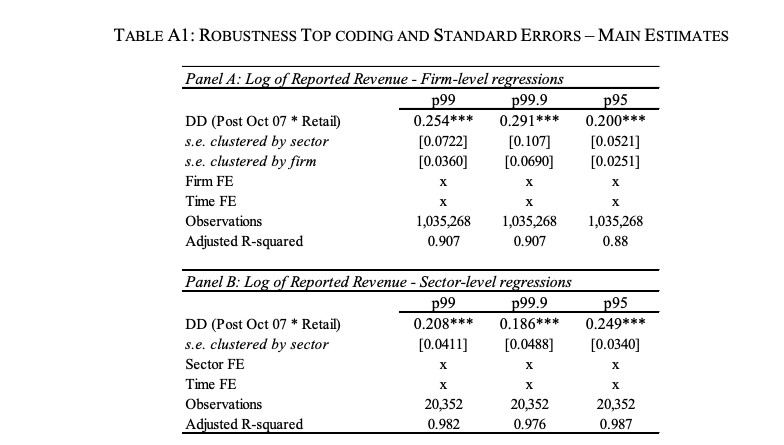
\includegraphics[width=\textwidth]{Paper Presentations/Consumers as Tax Auditors/R1.png}
\end{figure}
\end{frame}


\begin{frame}
\frametitle{Program Participation and Role of Incentives}
\begin{figure}
    \centering
    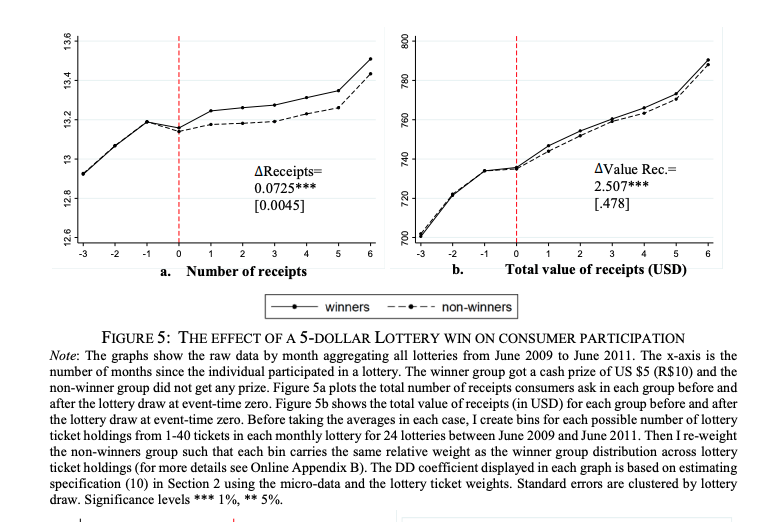
\includegraphics[width=\textwidth]{Paper Presentations/Consumers as Tax Auditors/F5.png}
\end{figure}
\end{frame}

\begin{frame}
\frametitle{Conclusions}
\begin{itemize}
\item Tax rates and enforcement are thus complementary levers. 
\item Jointly optimizing tax rates and
enforcement would lead to 26\% higher revenue gains than optimizing them independently.
\end{itemize}
\end{frame}

\end{document}
